%==============================================================================
% document template for a LaTeX file
% Created : 22.11.2006 by Romain de Wolff
% Modif : 18 janvier 2008, respect standart HEIG-VD pour travaux de diplômes
%==============================================================================
% configurations du document
\documentclass[a4paper, 11pt]{article}
\usepackage[utf8]{inputenc}
\usepackage[cyr]{aeguill}
\usepackage[frenchb]{babel}       % \og et \fg pour les guillemets
\usepackage{url}                          % pour inclure des URLs
\usepackage{color}                      % utilisé pour le code source
\usepackage{listings}                   % pour inclure le code source
\usepackage{geometry}          	  % pour les marges
%\usepackage{algorithmic}         % pour présenter les algos
%\usepackage{algorithm}            % pour présenter les algos
\usepackage{graphicx}                 % pour inclure des images
\usepackage{fancyvrb}                 % pour avoir du verbatim encadré
\usepackage{url}                           % pour inclure des URLs
\usepackage{geometry}               % See geometry.pdf to learn the layout options
\usepackage{moreverb}				   % permet d'encadrer le verbatim à l'aide de la commande \begin{boxedverbatim}
\usepackage{longtable}
\usepackage{courier}
\usepackage{color}

% color definitions
\definecolor{dkgreen}{rgb}{0,0.6,0}
\definecolor{gray}{rgb}{0.5,0.5,0.5}
\definecolor{lightblue}{rgb}{0.92,0.92,1}
 
\geometry{a4paper}                        % ... or a4paper or a5paper or ... 
%\geometry{landscape}                  % Activate for for rotated page geometry
\usepackage[parfill]{parskip}           % Activate to begin paragraphs with an empty line rather than an indent
%\usepackage{amssymb}
%\usepackage{epstopdf}                
\usepackage{bibtopic}				      % Pour créer des références divers (webographie, etc) 
\geometry{ hmargin=3.5cm, vmargin=2.5cm } % marges
%==============================================================================
% debut macro 
% permet de mettre en gros la premiere lettre d'un paragraphe
\font\capfont=cmbx12 at 44.87 pt % or yinit, or...?
\newbox\capbox \newcount\capl \def\a{A}
\def\docappar{\medbreak\noindent\setbox\capbox\hbox{%
\capfont\a\hskip0.15em}\hangindent=\wd\capbox%
\capl=\ht\capbox\divide\capl by\baselineskip\advance\capl by1%
\hangafter=-\capl%
\hbox{\vbox to8pt{\hbox to0pt{\hss\box\capbox}\vss}}}
\def\cappar{\afterassignment\docappar\noexpand\let\a }
% fin macro
%==============================================================================

\lstset{language=java,
  %keywords={break,case,catch,continue,else,elseif,end,for,function,
  %   global,if,otherwise,persistent,return,switch,try,while},
  basicstyle=\ttfamily\small,
  %basicstyle=\scriptsize, 
  keywordstyle=\color{blue},
  commentstyle=\color{dkgreen},
  stringstyle=\color{red},
  numbers=none,
  numberstyle=\tiny\color{gray},
  stepnumber=1,
  numbersep=10pt,
  backgroundcolor=\color{lightblue},
  tabsize=1,
  linewidth=0pt,
  showspaces=false,
  showstringspaces=false,
  frame=single,
  framexleftmargin=10pt,
  framexrightmargin=10pt,
  framexbottommargin=7pt,
  framextopmargin=7pt,
  linewidth=390pt, % largeur de la ligne de code affichée
  xleftmargin=10pt, % espace avant le debut du cadre
  aboveskip=20pt
}

%==============================================================================
% première page
\title{ %
\includegraphics[width=100px]{HEIG-VD.jpg} \\ \vspace{4cm}
\vspace{2cm}
\Huge{Laboratoire no2 - Voyageur de commerce} \\ \vspace{2.5cm} 
\small{dans le cadre du cours} \\
\vspace{1cm} 
\Large{Méthodes d'optimisation bio-inspirées}\\
\vspace{6cm}
\small{Auteurs}
} 

\author{Simon \bsc{Hintermann}, Romain \bsc{de Wolff} \\ IL2008 \\ \vspace{0.7cm} \\ 
Professeur: M. Éric \bsc{Taillard} \vspace{0.5cm}}
\date{Lausanne, le 2 avril 2008}  % Activate to display a given date or no date
\pagebreak{}

\begin{document}
\maketitle
\thispagestyle{empty} % enlève le numéro de page sur la page de titre (uniquement)
\newpage
%Table of contents
\tableofcontents
\newpage
%==============================================================================
% configuration des numérotations de pages (chiffres romains)
\pagenumbering{arabic} \setcounter{page}{1} 

% Configuration de la distance d'interligne 
{\setlength{\baselineskip}{1.2\baselineskip}
% Configuration de la distance entre les paragraphes
\parskip=10pt
%==============================================================================

%==============================================================================
\section{Introduction}
%==============================================================================

	Ce laboratoire porte sur le construction de chemin à l'aide d'une colonie de fourmis artificielle. Il s'agit de trouver une tournée la plus courte pour un ensemble donné de points avec des coordonnées. Il est possible de faire de la recherche locale pour améliorer les résultats trouvés par les fourmis, à l'aide d'un technique 2-opt ou 3-opt.

%==============================================================================
\section{Méthodes}
%==============================================================================

	La méthode utilisée est celle donnée dans le cours de m. Taillard, avec laquellle on simule le passage de plusieurs fourmis laissant des traces de phéromones. Ces traces vont inciter les fourmis à passer à l'endroit où le plus d'autres fourmis sont déjà passées, et ainsi favoriser le chemin le «plus court». Ce chemin ne sera bien sûr pas optimal en le considérant de manière globale, mais il sera quand même un bon début pour ensuite y ajouter une recherche locale en 2-opt ou en 3-opt, afin d'optimiser le travail des fourmis.

	Les fourmis sont envoyées par vagues pour trouver un bon chemin, en utilisant les traces globales et en mettant à jour leurs traces locales. Les traces locales sont mises à jour à la fin de chaque vague avec les traces locales des fourmis de la vague terminée. On va mémoriser le chemin parcouru par la dernière fourmi de chaque vague et calculer sa longueur. Le meilleur chemin sera représenté dans un fichier Postscript permettant de visualiser le parcours.

	Nous avons choisi de faire la recherche locale 2-opt pour optimiser le parcours de nos fourmis. Cette recherche locale va optimiser le parcours de chacune des fourmis. Une fois son parcours optimisé, les traces locales seront mises à jour avec le chemin optimisé. La boucle d'optimisation sera exécutée tant que des améliorations auront été possibles.

	Notre programme peut être lancé avec un paramètre représentant le nom du fichier à traiter, et si rien n'est mis, le programme prendra automatiquement \textit{BERLIN52.TSP}.

%==============================================================================
\section{Paramètres}
%==============================================================================

Les tests suivants ont été faits avec les paramètres suivants:

\begin{itemize}
	\item{}Fichier: \textit{Berlin52.TSP}
	\item{}$\alpha$: 1
	\item{}$\beta:$ 4
	\item{}Nombre de vagues: 500
	\item{}Q: 10
	\item{}Constante d'évaporation: 0.999
	\item{}Nombre de fourmis: 300
\end{itemize}
\medskip

	Tout d'abord, regardons comment se comporte notre algorithme sans les traces et sans le 2-opt. La figure \ref{fig:1} montre comment se comporte notre recherche de tournée: les résultats sont répartis entre environ 14'000 et 10'000 sans aucune tendance particulière.
	
\begin{figure}[H]
   \begin{center}
      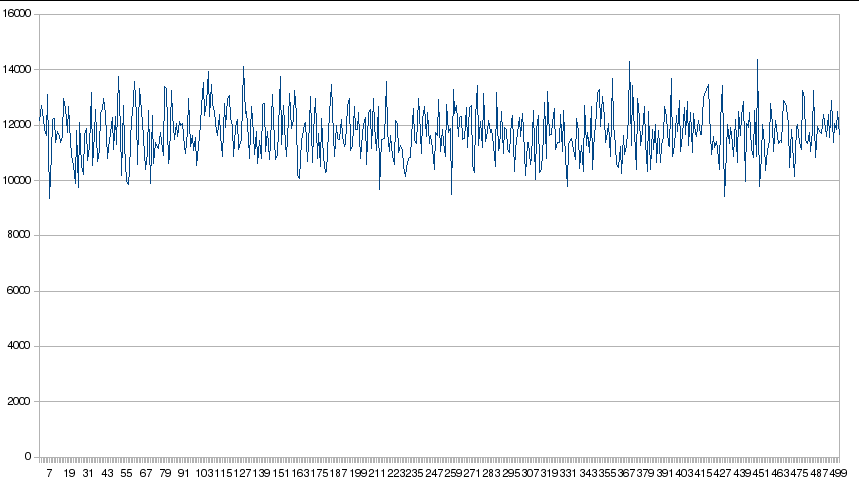
\includegraphics[width=14cm]{../images/1.png}
   \end{center}
   \caption{Comportement sans les traces}
	\label{fig:1}
\end{figure}

	Ensuite, ajoutons le principe des traces, et la figure \ref{fig:2} nous montre que, cette fois-ci, une tendance se dessine clairement au début, où l'on voit que la courbe descend assez vite (on aurait pu préciser le phénomène en réduisant le nombre de vagues). Au début du graphe, la moyenne est environ de 11'000, pour descendre très tôt (environ 100 vagues) autour des 9'500. Les solutions se trouvent entre 11'000 et 8'500 environ, ce qui est déjà bien mieux que notre version prenant en compte seulement les distances.

\begin{figure}[H]
   \begin{center}
      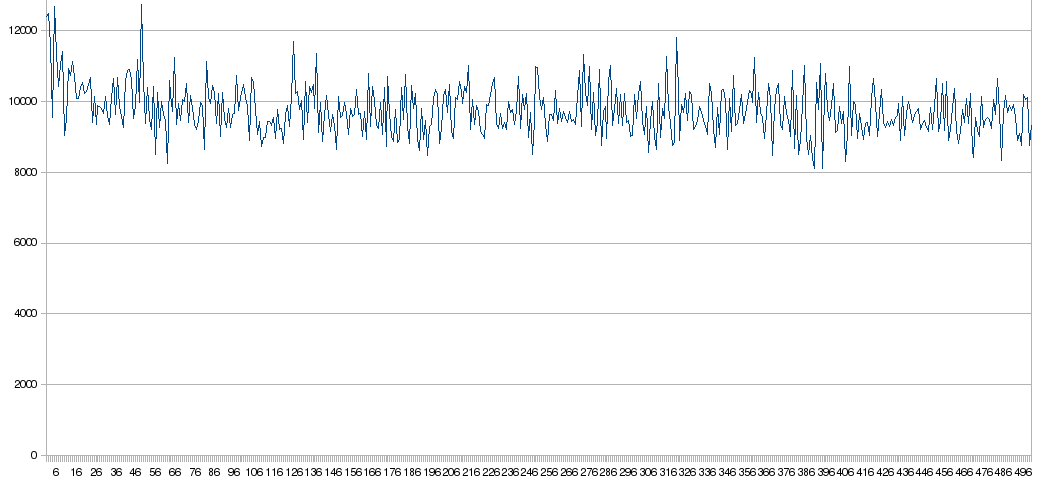
\includegraphics[width=14cm]{../images/2.png}
   \end{center}
   \caption{Comportement avec les traces}
	\label{fig:2}
\end{figure}

	Puis, finalement, on ajoute l'optimisation avec le 2-opt. Cette technique amène une grande amélioration dans la qualité de nos résultats. La figure \ref{fig:3} montre que nos solutions sont maintenant plutôt entre un peu moins de 8000 et 9'500.

\begin{figure}[H]
   \begin{center}
      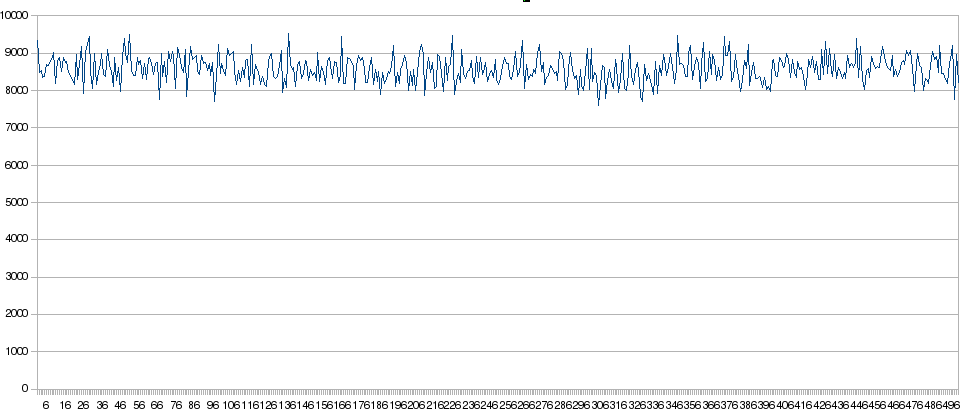
\includegraphics[width=14cm]{../images/3.png}
   \end{center}
   \caption{Comportement avec les traces et 2-opt}
	\label{fig:3}
\end{figure}

	Cette méthode de construction de tournées permet de trouver des résultats tout à fait corrects en un temps raisonnable, comme nous le montre la figure \ref{fig:4}, meilleure tournée que nous ayons trouvée pour le fichier \textit{Berlin52.TSP} (7544.37 de longueur).

\begin{figure}[H]
   \begin{center}
      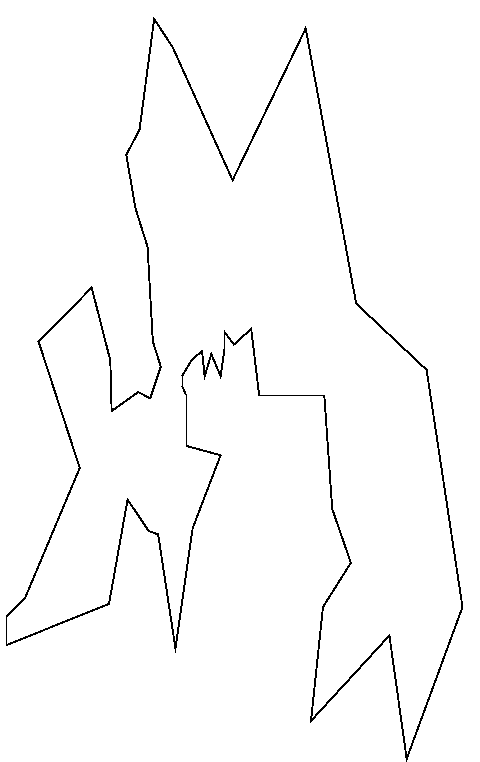
\includegraphics[width=14cm]{../images/4.png}
   \end{center}
   \caption{Meilleure tournée obtenue pour le fichier \textit{Berlin52.TSP}}
	\label{fig:4}
\end{figure}

	Essayons maintenant de faire changer certains paramètres pour trouver une bonne configuration.

	Si le paramètre $\beta$ est trop petit, la distance prendra plus d'importance que les traces, car cette distance est toujours au-dessous de zéro, et le fait de l'élever à une quelquonque puissance réduira sa force. La figure \ref{fig:5} ($\beta$=1) montre que, pour les mêmes paramètres qu'à la figure \ref{fig:3}, les résultats varient un peu plus haut, mais cette différence n'est pas flagrante.

\begin{figure}[H]
   \begin{center}
      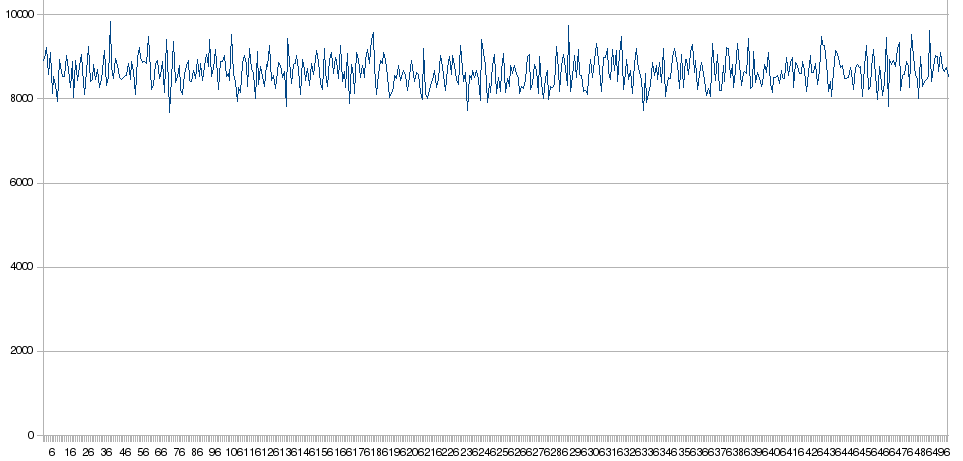
\includegraphics[width=14cm]{../images/5.png}
   \end{center}
   \caption{Résultats avec un $\beta$ de 1}
	\label{fig:5}
\end{figure}

	Au contraire, si $\beta$ est trop grand, les résultats auront tendance à réduire leur espace d'expression, comme le montre la figure \ref{fig:6} ($\beta$=10). On voit que les résultats descendent moins souvent au-dessous de la barre des 8'000.

\begin{figure}[H]
   \begin{center}
      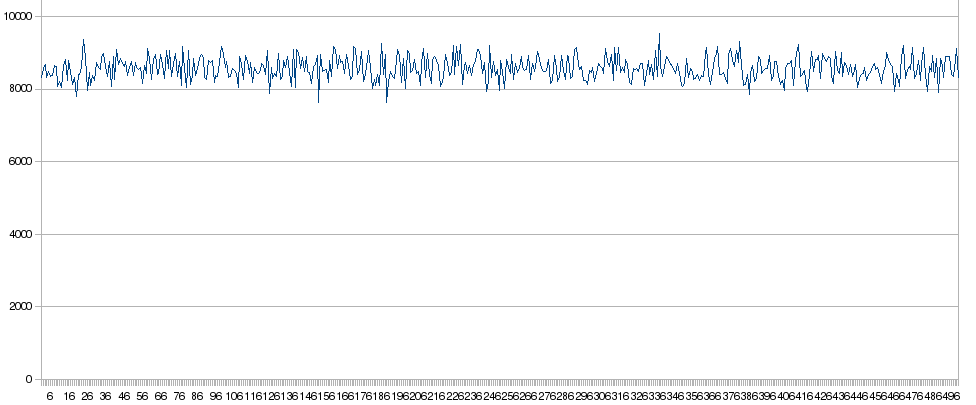
\includegraphics[width=14cm]{../images/6.png}
   \end{center}
   \caption{Résultats avec un $\beta$ de 10}
	\label{fig:6}
\end{figure}

	Le paramètre $\alpha$ réagitde la manière inverse. Ces deux paramètres doivent être plus ou moins réglés, mais ils ne sont pas vitaux. De plus, il faudra revoir leur valeur à chaque fois que l'on changera de fichier, car les valeurs qui seront bonnes pour un fichier contenant des distances entre 1'000 et 10'000 ne seront sûrement pas bonnes pour un fichier avec des distances entre 0.0001 et 0.01... il faudra donc revoir ces paramètres à chaque fois, ou régler le problème de manière dynamique en trouvant le rapport approximatif entre la valeur du terme $\tau^\alpha_{ij}$ et celle de $\eta^\beta_{ij}$.

	Le paramètre du nombre de vagues est important pour que les traces puissent être prises en compte, mais comme le montre la figure \ref{fig:2}, au bout de quelques dixaines de vagues, les résultats sont déjà bien meilleurs et varient par la suite dans la même fourchette. Le fait de mettre un grand nombre de vagues va simplement augmenter nos chances de trouver une bonne solution à la fin de l'exécution.

	La constante $Q$, utilisée dans la mise à jour des traces locales sert à pondérer le poids des traces laissés par les fourmis lors de chaque passage. Ce paramètre peut être modifié, mais il devra être en rapport avec $\alpha$ et la constante d'évaporation, nous avons donc décidé de ne pas faire des tests en changeant ce paramètre, il a été fixé à 10.

	La constante d'évaporation des traces  ne change pratiquement rien dans le cas où le 2-opt est appliqué et si on utilise le fichier Berlin52.TSP. On pourrait avancer que sur un autre fichier plus grand, cette constante aurait peut-être un autre impact.

	Si le nombre de fourmis est réduit, les traces évoluent moins vite, comme le montre la figure \ref{fig:7}, où on peut voir une descente progressive de la moyenne des résutats. Bien entendu, il ne sert à rien de mettre trop de fourmis, en tout cas pas dans le problème de \textit{BERLIN52.TSP}, car on ne ferait qu'augmenter le temps de calcul d'une vague. Nous avons mis le nombre de fourmis à 100, ce qui est peut-être déjà trop.

\begin{figure}[H]
   \begin{center}
      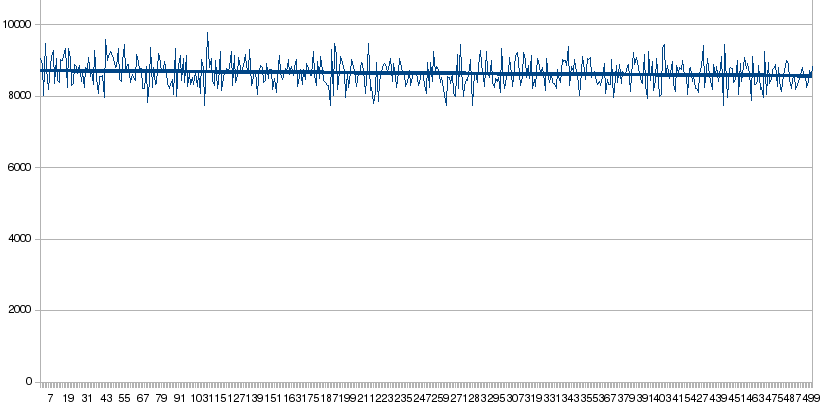
\includegraphics[width=14cm]{../images/7.png}
   \end{center}
   \caption{Résultats avec 10 fourmis}
	\label{fig:7}
\end{figure}

	La constante $t0$ utilisée pour initialiser la matrice des traces doit être plus grande que zéro, mais sa valeur importe peu, il suffit de la mettre à 0.1.

\subsection{Les autres fichiers}
	Le fichier \textit{BIER127.TSP}, par exemple, contient plus de données que \textit{BERLIN52.TSP}. Voyons ce que donne la même configuration qu'avant pour ce fichier. La figure \ref{fig:8} donne un exemple d'une tournée pour ce fichier.

\begin{figure}[H]
   \begin{center}
      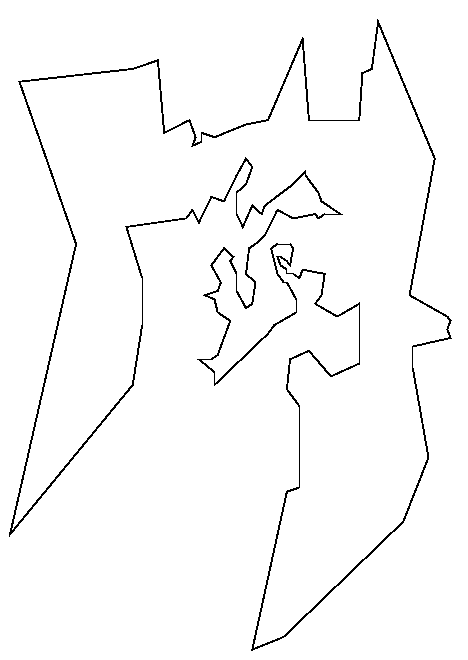
\includegraphics[width=14cm]{../images/8.png}
   \end{center}
   \caption{Tournée pour le fichier \textit{BIER127.TSP}}
	\label{fig:8}
\end{figure}

	La figure \ref{fig:9} donne l'évolution des solutions sur 500 vagues et 100 fourmis par vague. On voit bien que la moyenne des solutions baisse au fur et à mesure des vagues. Il faudrait donc essayer de mettre plus de fourmis pour voir si les solutions seraient tout de suite meilleures. La figure \ref{fig:10} donne cette évolution, et on remarque que la moyenne des solutions descend plus vite et finit à une valeur plus basse que celle de la figure précédente. Augmenter le nombre de fourmis est donc une bonne idée. 

\begin{figure}[H]
   \begin{center}
      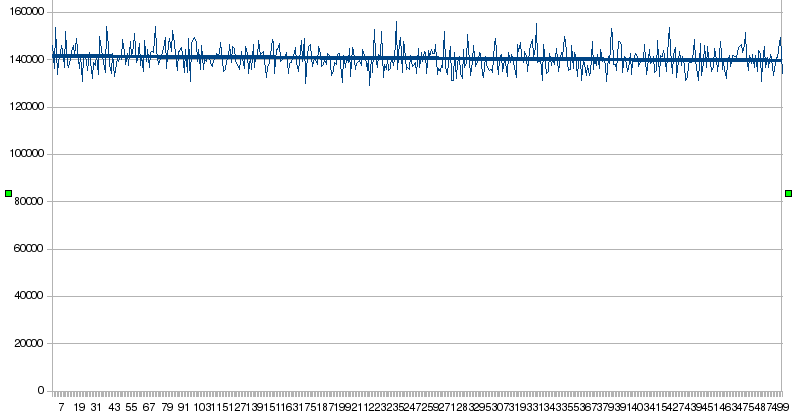
\includegraphics[width=14cm]{../images/9.png}
   \end{center}
   \caption{Evolution des solutions pour \textit{BIER127.TSP} avec 100 fourmis}
	\label{fig:9}
\end{figure}

\begin{figure}[H]
   \begin{center}
      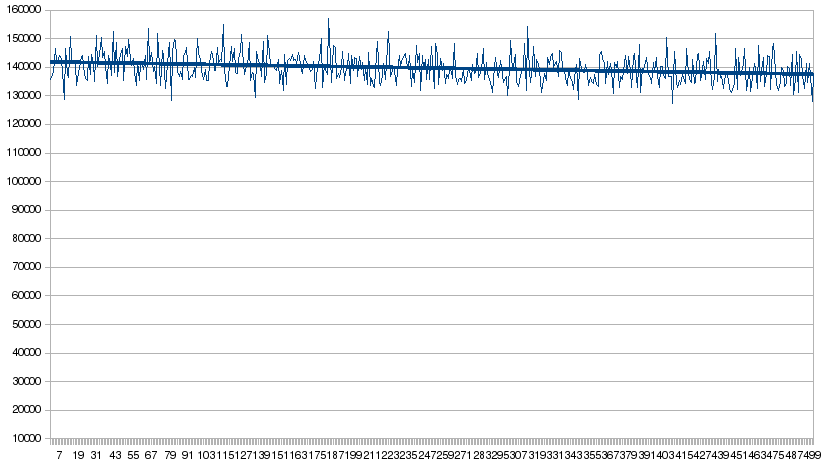
\includegraphics[width=14cm]{../images/10.png}
   \end{center}
   \caption{Evolution des solutions pour \textit{BIER127.TSP} avec 300 fourmis}
	\label{fig:10}
\end{figure}

	Mais ne nous arrêtons pas là, car il y a un autre facteur intéressant à prendre en compte: les distances; dans le fichier \textit{BIER127.TSP}, elles sont 10 fois supérieures à celles du fichier \textit{BERLIN52.TSP}. Il faudrait donc essayer de changer la valeur de la constante $Q$, par exemple, pour travailler avec les mêmes valeurs qu'avec \textit{BERLIN52.TSP}... Si on relance l'exécution avec 100 fourmis, mais une valeur de $Q$ 10 fois supérieure à celle utilisée pour \textit{BERLIN52.TSP}, c'est-à-dire 100, notre moyenne des solutions va effectivement se voir un peu améliorée, comme le montre la figure \ref{fig:11}.

\begin{figure}[H]
   \begin{center}
      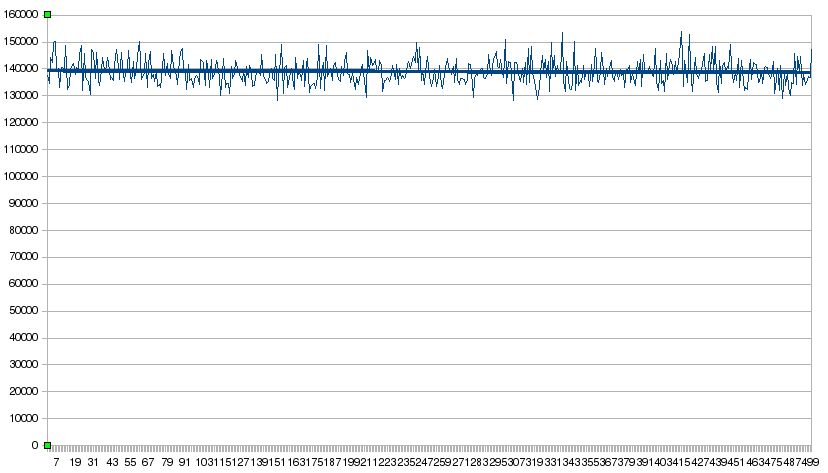
\includegraphics[width=14cm]{../images/11.png}
   \end{center}
   \caption{Evolution des solutions pour \textit{BIER127.TSP} avec 100 fourmis et $Q$=100}
	\label{fig:11}
\end{figure}

	Nous ne nous sommes pas intéressés aux autres fichiers, qui demandaient des temps de calcul assez prohibitifs pour pouvoir montrer quelque chose d'intéressant, mais il faudrait appliquer le même principe que ci-dessus en passant de \textit{BERLIN52.TSP} à \textit{BIER127.TSP}, c'est-à-dire modifier les paramètres en fonction des distances afin d'obtenir des bonnes solutions assez vite.

\subsection{Complexité}

	La boucle principale permettant aux fourmis de trouver une tournée est en O($m * n * v$), sans le 2-opt, où $m$ est le nombre de vagues, $n$ le nombre de fourmis et $v$ le nombre de villes. La sélection aléatoire d'une ville pour la construction du chemin est réalisée par la même technique utilisée lors du laboratoire précédent: la roulette. Les villes sélectionnées sont triées au début du tableau représentant ce chemin, laissant les villes non-sélectionnées à la fin du tableau, que l'on pourra reprendre à l'aide d'un index dynamique pour la sélection aléatoire. Cette manière de faire nous évite de devoir tenir une liste des villes déjà visitées.

	Le 2-opt, quant à lui, rajoute pas mal de complexité pour la construction du chemin. Il faut boucler deux fois sur v (O($v^2$)) (en réalité, cette estimation est fausse, car la deuxième boucle fait de moins en moins d'itéations...), et nous avons de plus décidé de refaire la double boucle tant que des modifications avaient été trouvées, ce qui pourrait de nouveau dégénérer en v, voire plus, mais nous allons prendre v comme valeur théorique maximale, dans le pire des cas. De plus, si la distance est plus courte pour la combinaison testée, on doit aller inverser le chemin entre les deux bornes. Pour inverser ce chemin, nous inversons le chemin le plus court, afin de limiter un peu le calcul. Cette inversion demande donc $nbVilles / 4$ passages dans la boucle d'inversion au pire. La complexité est donc de: O($v^{13/4}$) pour notre algorithme de recherche locale.

	La complexité globale de notre programme est donc de: O($m * n * v^{17/4}$), ce qui peut engendrer des temps de calcul assez prohibitifs pour les jeux de données étendus.

\subsection{Remarques} 

	Tous les graphiques présentés ont pour axe des x les itérations et la longueur de la tournée pour l'axe des y.

%==============================================================================
\section{Conclusion}
%==============================================================================

	Nous avons pris du plaisir à faire ce laboratoire, qui nous a permis de mettre en pratique la fameuse méthode du 2-opt vue en première année, et qui s'est avérée très utile dans ce cas. Nous sommes assez content de notre implémentation, qui nous paraît optimale au niveau de la complexité.

\end{document}